\chapter{Consuntivo}\label{Consuntivo}
Di seguito vengono indicate le spese sostenute dal gruppo confrontandole con quanto preventivato. Il bilancio potrà essere:
\begin{itemize}
	\item positivo: la spesa effettiva è minore di quanto preventivato;
	\item pari: la spesa effettiva è uguale a quanto preventivato;
	\item negativo: la spesa effettiva è maggiore di quanto preventivato.
\end{itemize}
\section{Periodo di analisi}\label{ConsuntivoPeriodoDiAnalisi}
Le ore di lavoro che sono state sostenute durante la fase di analisi sono considerate come ore di investimento e per questo motivo esse non vengono rendicontate.
\quad
\def\tabularxcolumn#1{m{#1}}
{\rowcolors{2}{RawSienna!90!RawSienna!20}{RawSienna!70!RawSienna!40}
	\begin{center}
		\renewcommand{\arraystretch}{1.4}
		\begin{tabularx}{10cm}{|X|c|c|}
			\hline
			\rowcolor{airforceblue}
			\textbf{Ruolo} & \textbf{Ore} & \textbf{Costo}\\
			\hline
			Responsabile & 26(+0) & 780\euro(+0\euro)\\
			\hline
			Amministratore & 42(+0) & 840\euro(+0\euro)\\
			\hline
			Analista & 49(+15) & 1225\euro(+375\euro)\\
			\hline
			Progettista & 0(+0) & 0\euro(+0\euro)\\
			\hline
			Programmatore & 0(+0) & 0\euro(+0\euro)\\
			\hline
			Verificatore & 33(+10) & 495\euro(+150\euro)\\
			\hline
			\textbf{Totale Preventivo} & \textbf{150} & \textbf{3340\euro}\\
			\hline
			\textbf{Totale Consuntivo} & \textbf{175} & \textbf{3865\euro}\\
			\hline
			\textbf{Differenza} & \textbf{25} & \textbf{525\euro}
		\end{tabularx}
		\captionof{table}{\textbf{Consuntivo della fase di Analisi}}
	\end{center}

\subsection{Conclusioni}\label{ConsuntivoPeriodoDiAnalisiConclusioni}
Come emerso dalla tabella precedente, il bilancio risulta negativo in quanto il gruppo ha ritenuto necessario impiegare più tempo del previsto nei ruoli di \textit{Analista} e \textit{Verificatore}. I motivi di tale ritardo sono:
\begin{itemize}
	\item la complessità nell'individuazione dei requisiti;
	\item la grande quantità di lavoro nel revisionare i documenti. Infatti, trattandosi di un processo nuovo, ogni componente ha dovuto imparare a svolgerlo in maniera corretta, efficacie ed efficiente.
\end{itemize}

\subsection{Preventivo a finire}\label{ConsuntivoPeriodoDiAnalisiPreventivoAFinire}
Il preventivo a finire, nonostante in questa fase siano state necessarie più ore del previsto, è in linea con quanto descritto nella sezione precedente. Il gruppo non ritiene il surplus di 500\euro{} un problema in quanto le ore lavorative e i costi sostenuti in questa fase non verranno rendicontati. Per questo motivo il gruppo ha deciso di non prendere alcuna contromisura nella pianificazione futura.

\section{Periodo di consolidamento dei requisiti}\label{ConsuntivoPeriodoDiConsolidamentoDeiRequisiti}
Le ore di lavoro calcolate per questo periodo sono considerate come ore di investimento e, per tale motivo, non vengono rendicontate.

\quad
\def\tabularxcolumn#1{m{#1}}
{\rowcolors{2}{RawSienna!90!RawSienna!20}{RawSienna!70!RawSienna!40}
	\begin{center}
		\renewcommand{\arraystretch}{1.4}
		\begin{tabularx}{10cm}{|X|c|c|}
			\hline
			\rowcolor{airforceblue}
			\textbf{Ruolo} & \textbf{Ore} & \textbf{Costo}\\
			\hline
			Responsabile & 4(+0) & 120\euro(+0\euro)\\
			\hline
			Amministratore & 8(+0) & 160\euro(+0\euro)\\
			\hline
			Analista & 4(+0) & 100\euro(+0\euro)\\
			\hline
			Progettista & 0(+0) & 0\euro(+0\euro)\\
			\hline
			Programmatore & 0(+0) & 0\euro(+0\euro)\\
			\hline
			Verificatore & 8(0) & 120\euro(+0\euro)\\
			\hline
			\textbf{Totale Preventivo} & \textbf{24} & \textbf{500\euro}\\
			\hline
			\textbf{Totale Consuntivo} & \textbf{24} & \textbf{500\euro}\\
			\hline
			\textbf{Differenza} & \textbf{0} & \textbf{0\euro}
		\end{tabularx}
		\captionof{table}{\textbf{Consuntivo della fase di Consolidamento dei requisiti}}
	\end{center}

\subsection{Conclusioni}\label{ConsuntivoPeriodoDiConsolidamentoDeiRequisitiConclusioni}
Grazie al minor carico di lavoro, le ore preventivate sono state rispettate quindi non è presente alcuna differenza rispetto alle ore effettive di lavoro. Inoltre il gruppo è riuscito a procedere senza alcun problema con lo studio personale per lo svolgimento della fase successiva del lavoro.

\subsection{Preventivo a finire}\label{ConsuntivoPeriodoDiConsolidamentoDeiRequisitiPreventivoAFinire}
Poichè le ore di lavoro previste sono state rispettate, il preventivo a finire risulta coerente con quello previsto.

\section{Periodo di progettazione architetturale}\label{ConsuntivoPeriodoDiProgettazioneArchitetturale}

Il gruppo ha suddiviso questa fase in diversi periodi per organizzare al meglio il lavoro, di conseguenza il consuntivo viene analizzato in funzione di ogni sua parte.

\subsection{Primo periodo - dal 2021-01-19 al 2021-02-15}\label{ConsuntivoPeriodoDiProgettazioneArchitetturaleIncrementoEVerifica}

Le ore dedicate in questo periodo sono atte al completamento della fase di Incremento e Verifica descritta nella \S~\ref{PianificazioneProgettazioneArchitetturale} e a formazione personale sulle tecnologie da utilizzare per lo sviluppo della Technology Baseline$_{\scaleto{G}{3pt}}$.

\quad
\def\tabularxcolumn#1{m{#1}}
{\rowcolors{2}{RawSienna!90!RawSienna!20}{RawSienna!70!RawSienna!40}
	\begin{center}
		\renewcommand{\arraystretch}{1.4}
		\begin{tabularx}{10cm}{|X|c|c|}
			\hline
			\rowcolor{airforceblue}
			\textbf{Ruolo} & \textbf{Ore} & \textbf{Costo}\\
			\hline
			Responsabile & 7(+0) & 210\euro(+0\euro)\\
			\hline
			Amministratore & 7(+0) & 140\euro(+0\euro)\\
			\hline
			Analista & 8(+10) & 200\euro(+250\euro)\\
			\hline
			Progettista & 2(+0) & 44\euro(+0\euro)\\
			\hline
			Programmatore & 0(+0) & 0\euro(+0\euro)\\
			\hline
			Verificatore & 15(+10) & 225\euro(+150\euro)\\
			\hline
			\textbf{Totale Preventivo} & \textbf{39} & \textbf{819\euro}\\
			\hline
			\textbf{Totale Consuntivo} & \textbf{59} & \textbf{1219\euro}\\
			\hline
			\textbf{Differenza} & \textbf{20} & \textbf{400\euro}
		\end{tabularx}
		\captionof{table}{\textbf{Consuntivo del primo periodo}}
	\end{center}

\subsubsection{Conclusioni}
Come emerso dalla tabella precedente, il bilancio risulta negativo in quanto il gruppo ha ritenuto necessario impiegare più tempo del previsto nel ruolo di \textit{Verificatore} e di \textit{Analista}, per via l'esigenza di correggere alcuni errori sollevati in seguito alla Revisione dei Requisiti.
%(voglio dire che abbiamo corretto i difetti gravi segnalati da tullio ed è per questo che il verificatore ha queste ore in più ma non so come dirlo in modo carino e formale)

\subsubsection{Preventivo a finire}
Il preventivo a finire presenta un surplus di 400\euro. Per questo motivo il gruppo ha deciso di tamponare il problema cercando di rispettare le ore preventivate nelle fasi successive in modo tale da non sforare troppo dal preventivo inizialmente previsto.

\subsection{Secondo periodo - dal 2021-02-16 al 2021-03-04 }\label{ConsuntivoPeriodoDiProgettazioneArchitetturaleTechnologyBaselinePrimoIncremento}

Le ore dedicate in questo periodo sono atte al completamento del primo incremento descritto nella  \S~\ref{PianificazioneProgettazioneArchitetturale}.

\quad
\def\tabularxcolumn#1{m{#1}}
{\rowcolors{2}{RawSienna!90!RawSienna!20}{RawSienna!70!RawSienna!40}
	\begin{center}
		\renewcommand{\arraystretch}{1.4}
		\begin{tabularx}{10cm}{|X|c|c|}
			\hline
			\rowcolor{airforceblue}
			\textbf{Ruolo} & \textbf{Ore} & \textbf{Costo}\\
			\hline
			Responsabile & 9(+0) & 270\euro(+0\euro)\\
			\hline
			Amministratore & 10(+0) & 200\euro(+0\euro)\\
			\hline
			Analista & 11(+0) & 275\euro(+0\euro)\\
			\hline
			Progettista & 54(+15) & 1188\euro(+330\euro)\\
			\hline
			Programmatore & 7(+0) & 105\euro(+0\euro)\\
			\hline
			Verificatore & 20(+0) & 300\euro(+0\euro)\\
			\hline
			\textbf{Totale Preventivo} & \textbf{111} & \textbf{2338\euro}\\
			\hline
			\textbf{Totale Consuntivo} & \textbf{126} & \textbf{2668\euro}\\
			\hline
			\textbf{Differenza} & \textbf{15} & \textbf{330\euro}
		\end{tabularx}
		\captionof{table}{\textbf{Consuntivo del secondo periodo}}
	\end{center}

\subsubsection{Conclusioni}
Come emerso dalla tabella precedente, il bilancio risulta negativo in quanto il gruppo ha ritenuto necessario impiegare più tempo del previsto nel ruolo di \textit{Progettista}. Il motivo di ciò è la mole di lavoro inaspettata che ha dovuto ricoprire questo ruolo per l'acerbità dei componenti riguardo alle tecnologie da utilizzare.

\subsubsection{Preventivo a finire}
Il preventivo a finire presenta un surplus di 330\euro. Per cercare di rientrare nelle ore prestabilite per le consegne successive, il gruppo ha deciso di organizzare meglio lo studio individuale di ognuno e di migliorare la comunicazione interna: in questo modo, quando emerge un problema, questo può essere risolto non dal singolo, che potrebbe impiegarci troppo tempo, ma dal gruppo.

\subsection{Terzo periodo - dal 2021-03-05 al 2021-03-15}\label{ConsuntivoPeriodoDiProgettazioneArchitetturaleTechnologyBaselineTerzoIncremento}

Le ore dedicate in questo periodo sono atte al completamento del secondo incremento descritto nella \S~\ref{PianificazioneProgettazioneArchitetturale}.

\quad
\def\tabularxcolumn#1{m{#1}}
{\rowcolors{2}{RawSienna!90!RawSienna!20}{RawSienna!70!RawSienna!40}
	\begin{center}
		\renewcommand{\arraystretch}{1.4}
		\begin{tabularx}{10cm}{|X|c|c|}
			\hline
			\rowcolor{airforceblue}
			\textbf{Ruolo} & \textbf{Ore} & \textbf{Costo}\\
			\hline
			Responsabile & 8(+0) & 240\euro(+0\euro)\\
			\hline
			Amministratore & 9(+0) & 180\euro(+0\euro)\\
			\hline
			Analista & 10(+0) & 250\euro(+0\euro)\\
			\hline
			Progettista & 30(+5) & 660\euro(+150\euro)\\
			\hline
			Programmatore & 5(+0) & 75\euro(+0\euro)\\
			\hline
			Verificatore & 19(+0) & 285\euro(+0\euro)\\
			\hline
			\textbf{Totale Preventivo} & \textbf{81} & \textbf{1690\euro}\\
			\hline
			\textbf{Totale Consuntivo} & \textbf{86} & \textbf{1840\euro}\\
			\hline
			\textbf{Differenza} & \textbf{5} & \textbf{150\euro}
		\end{tabularx}
		\captionof{table}{\textbf{Consuntivo del terzo periodo}}
	\end{center}

\subsubsection{Conclusioni}
Come emerso dalla tabella il bilancio risulta essere negativo in quanto il gruppo ha ritenuto necessario impiegare più tempo del previsto nel ruolo di \textit{Progettista} dovuto alla mole di lavoro legata al secondo incremento e alla conclusione dei documenti da presentare per la Revisione di Progettazione.

\subsubsection{Preventivo a finire}
Il preventivo a finire presenta un surplus di 150\euro. Per cercare di rientrare nelle ore prestabilite il gruppo ha lavorato in modo tale da avvantaggiarsi con il lavoro della fase successiva.

\subsection{Consuntivo complessivo delle fasi}\label{ConsuntivoPeriodoDiProgettazioneArchitetturaleConsuntivoComplessivoDelleFasi}

Nella tabella successiva viene descritto il calcolo delle ore totali di tutte le parti precedentemente descritte.

\quad
\def\tabularxcolumn#1{m{#1}}
{\rowcolors{2}{RawSienna!90!RawSienna!20}{RawSienna!70!RawSienna!40}
	\begin{center}
		\renewcommand{\arraystretch}{1.4}
		\begin{tabularx}{10cm}{|X|c|c|}
			\hline
			\rowcolor{airforceblue}
			\textbf{Ruolo} & \textbf{Ore} & \textbf{Costo}\\
			\hline
			Responsabile & 24(+0) & 720\euro(+0\euro)\\
			\hline
			Amministratore & 26(+0) & 520\euro(+0\euro)\\
			\hline
			Analista & 29(+10) & 725\euro(+250\euro)\\
			\hline
			Progettista & 86(+20) & 1892\euro(+440\euro)\\
			\hline
			Programmatore & 12(+0) & 180\euro(+0\euro)\\
			\hline
			Verificatore & 54(+10) & 810\euro(+150\euro)\\
			\hline
			\textbf{Totale Preventivo} & \textbf{231} & \textbf{4847\euro}\\
			\hline
			\textbf{Totale Consuntivo} & \textbf{271} & \textbf{5687\euro}\\
			\hline
			\textbf{Differenza} & \textbf{40} & \textbf{840\euro}
		\end{tabularx}
		\captionof{table}{\textbf{Consuntivo complessivo delle fasi}}
	\end{center}

\subsection{Conclusioni}\label{ConsuntivoPeriodoDiProgettazioneArchitetturaleConclusioni}
Il bilancio, come emerge dalla tabella precedente, risulta negativo poiché il gruppo ha ritenuto necessario impiegare più ore nei ruoli di \textit{Progettista},\textit{Verificatore} e \textit{Analista}. I motivi di tale ritardo sono:
\begin{itemize}
	\item il tempo impiegato per la correzione e l'aggiornamento dei documenti si è rivelato essere più di quello preventivato;
	\item trattandosi di un progetto complesso ed articolato, con tecnologie nuove ad ogni componente del gruppo, la parte di progettazione si è rivelata molto più complicata del previsto.
\end{itemize}

\subsection{Preventivo a finire}\label{ConsuntivoPeriodoDiProgettazioneArchitetturalePreventivoAFinire}
Il preventivo a finire risulta quindi con un surplus di 840\euro. Dalle analisi fatte riguardo ai preventivi a finire di ogni parte di questa fase il gruppo ha rilevato che:
\begin{itemize}
	\item deve essere presente un'organizzazione migliore nella verifica e validazione dei documenti;
	\item lo studio personale delle tecnologie deve essere più efficiente in modo da poter sviluppare in maniera più proficua;
	\item il miglioramento delle comunicazioni interne al gruppo può essere una parte fondamentale nella risoluzione di possibili problemi che emergono nel corso dello sviluppo del progetto.
\end{itemize}
Se ogni componente cerca di perseguire questi tre obiettivi il surplus presente in questo preventivo non risulterà un problema per l'ideazione del progetto. Inoltre per cercare di sopperire le ore aggiuntive il gruppo ha cercato di avanzare il più possibile con lo sviluppo dell'applicazione per non gravare troppo nelle fasi successive.

\section{Periodo di progettazione di dettaglio e codifica}\label{ConsutivoFaseProgettazioneDettaglioCodifica}
Il gruppo ha suddiviso questa fase in diversi periodi ai quali sono stati assegnati uno o più incrementi per organizzare al meglio il lavoro, di conseguenza il consuntivo viene analizzato in funzione di ogni incremento relativo ad ogni periodo.

\subsection{Primo periodo - dal 2021-03-15 al 2021-03-22}\label{ConsuntivoPrimoPeriodoDiProgettazioneDiDettaglioCodifica}

\subsubsection{Bilancio degli incrementi}\label{ConsuntivoPrimoPeriodoDiProgettazioneDiDettaglioCodificaIncrementi}

La seguente tabella indica le ore effettivamente investite in ogni ruolo per il completamento di ciascun incremento di questo periodo e la differenza con quelle preventivate.

\quad
\def\tabularxcolumn#1{m{#1}}
{\rowcolors{2}{RawSienna!90!RawSienna!20}{RawSienna!70!RawSienna!40}

	\begin{center}
		\renewcommand{\arraystretch}{1.4}
		\begin{tabularx}{\textwidth}{|X|c|c|c|c|c|c|c|}
			\hline
			\rowcolor{airforceblue}
			\textbf{Incremento} & \textbf{Re} & \textbf{Am} & \textbf{An} & \textbf{Pt} & \textbf{Pr} & \textbf{Ve} & \textbf{Totale ore}\\
			\hline
			\textit{Incremento 1} & 5(+0) & 8(+5) & 0(-19) & 5(+0) & 0(+0) & 14(+0) & 32(-14) \\
			\hline
			\textit{Incremento 2} & 3(+0) & 3(+3) & 0(+0) & 15(+0) & 25(+5) & 0(+0) & 46(+8)\\
			\hline
			Totale ore ruolo & 8(+0) & 11(+8) & 19(+0) & 20(+0) & 25(+5) & 14(+0) & 78(-6)\\
			\hline
		\end{tabularx}
		\captionof{table}{\textbf{Ore risultanti degli incrementi del primo periodo della fase di Progettazione di dettaglio e codifica}}
	\end{center}

\subsubsection{Consuntivo}\label{ConsuntivoPrimoPeriodoDiProgettazioneDiDettaglioCodificaIncrementiCosto}

\quad
\def\tabularxcolumn#1{m{#1}}
{\rowcolors{2}{RawSienna!90!RawSienna!20}{RawSienna!70!RawSienna!40}
	\begin{center}
		\renewcommand{\arraystretch}{1.4}
		\begin{tabularx}{10cm}{|X|c|c|}
			\hline
			\rowcolor{airforceblue}
			\textbf{Ruolo} & \textbf{Ore} & \textbf{Costo}\\
			\hline
			Responsabile & 8(+0) & 240\euro(+0\euro)\\
			\hline
			Amministratore & 11(+8) & 220\euro(+160\euro)\\
			\hline
			Analista & 0(-19) & 0\euro(-475\euro)\\
			\hline
			Progettista & 20(+0) & 440\euro(+0\euro)\\
			\hline
			Programmatore & 25(+5) & 375\euro(+75\euro)\\
			\hline
			Verificatore & 14(+0) & 210\euro(+0\euro)\\
			\hline
			\textbf{Totale Preventivo} & \textbf{84} & \textbf{1725\euro}\\
			\hline
			\textbf{Totale Consuntivo} & \textbf{78} & \textbf{1485\euro}\\
			\hline
			\textbf{Differenza} & \textbf{-6} & \textbf{-240\euro}
		\end{tabularx}
		\captionof{table}{\textbf{Consuntivo del primo periodo}}
	\end{center}

\subsubsection{Conclusioni}\label{ConsuntivoPrimoPeriodoDiProgettazioneDiDettaglioCodificaConclusioni}
	Come emerso dalla tabella precedente, il bilancio per questo periodo risulta positivo in quanto è stato impiegato meno tempo del previsto per il ruolo di \textit{Analista}, erroneamente preventivato nell' incremento 1 dato che per le modifiche all'\textit{Analisi dei Requisiti} si è deciso di aspettare la valutazione e le indicazioni del committente$_G$.
	Invece nel ruolo di \textit{Amministratore} sono state impiegate più ore perché c'è stato molto lavoro per ristrutturare il codice prodotto per il Proof of Concecpt$_G$ e questa figura è indispensabile per l'efficienza e l'operatività dell'ambiente di sviluppo.

\subsubsection{Ragionamento sugli scostamenti}\label{ConsuntivoPrimoPeriodoDiProgettazioneDiDettaglioCodificaRagionamentoScostamenti}
	Quello che emerge dagli scostamenti tra le ore preventivate e quelle in consuntivo fa notare subito che le ore preventivate in più nel ruolo di \textit{Analista} potevano essere evitate con uno studio più approfondito in fase di pianificazione.
	Per quanto riguarda il ruolo di \textit{Amministratore} invece risultano più ore in quanto si è deciso di andare il più avanti possibile con la codifica, sperando di poterle recuperare nei periodi successivi.


\subsubsection{Preventivo a finire}\label{ConsuntivoPrimoPeriodoDiProgettazioneDiDettaglioCodificaPreventivoFinire}
	Il preventivo a finire di questo primo periodo presenta una diminuzione di 240\euro, il che è un dato positivo se preso singolarmente ma, nel nostro caso, le ore mancanti potrebbero aggiungersi al periodo successivo. Terremo monitorato il lavoro per riuscire a mantenere il risparmio maturato in questo periodo per tutta la fase di Progettazione di dettaglio e codifica.

\subsection{Secondo periodo - dal 2021-03-23 al 2021-04-06 }\label{ConsuntivoSecondoPeriodoDiProgettazioneDiDettaglioCodifica}

\subsubsection{Bilancio degli incrementi}\label{ConsuntivoSecondoPeriodoDiProgettazioneDiDettaglioCodificaIncrementi}

	La seguente tabella indica le ore effettivamente investite in ogni ruolo per il completamento di ciascun incremento di questo periodo e la differenza con quelle preventivate.

\quad
\def\tabularxcolumn#1{m{#1}}
{\rowcolors{2}{RawSienna!90!RawSienna!20}{RawSienna!70!RawSienna!40}

	\begin{center}
		\renewcommand{\arraystretch}{1.4}
		\begin{tabularx}{\textwidth}{|X|c|c|c|c|c|c|c|}
			\hline
			\rowcolor{airforceblue}
			\textbf{Incremento} & \textbf{Re} & \textbf{Am} & \textbf{An} & \textbf{Pt} & \textbf{Pr} & \textbf{Ve} & \textbf{Totale ore}\\
			\hline
			\textit{Incremento 3} & 2(+0) & 3(+0) & 0(+0) & 7(+0) & 16(+3) & 0(+0) & 28(+3)\\
			\hline
			\textit{Incremento 4} & 8(+3) & 6(+0) & 14(+7) & 0(+0) & 0(+0) & 20(+4) & 48(+14) \\
			\hline
			\textit{Incremento 5} & 2(+0) & 4(+0) & 0(+0) & 11(+0) & 21(+3) & 0(+0) & 38(+3)\\
			\hline
			\textit{Incremento 6} & 1(+0) & 2(+0) & 0(+0) & 2(+0) & 4(+0) & 0(+0) & 9(+0)\\
			\hline
			\textit{Incremento 7} & 1(+0) & 2(+0) & 0(+0) & 1(+0) & 3(+0) & 0(+0) & 7(+0)\\
			\hline
			\textit{Incremento 8} & 5(+0) & 6(+0) & 0(+0) & 5(+0) & 13(+0) & 0(+0) & 29(+0)\\
			\hline
			\textit{Incremento 9} & 8(+2) & 7(+0) & 0(+0) & 13(+0) & 0(+0) & 16(+0) & 44(+2)\\
			\hline
			Totale ore ruolo & 27(+5) & 30(+0) & 14(+7) & 39(+0) & 57(+6) & 36(+4) & 203(+22)\\
			\hline
		\end{tabularx}
		\captionof{table}{\textbf{Ore risultanti degli incrementi del secondo periodo della fase di Progettazione di dettaglio e codifica}}
	\end{center}

\subsubsection{Consuntivo}\label{ConsuntivoSecondoPeriodoDiProgettazioneDiDettaglioCodificaIncrementiCosto}

	\quad
	\def\tabularxcolumn#1{m{#1}}
	{\rowcolors{2}{RawSienna!90!RawSienna!20}{RawSienna!70!RawSienna!40}
		\begin{center}
			\renewcommand{\arraystretch}{1.4}
			\begin{tabularx}{10cm}{|X|c|c|}
				\hline
				\rowcolor{airforceblue}
				\textbf{Ruolo} & \textbf{Ore} & \textbf{Costo}\\
				\hline
				Responsabile & 27(+5) & 810\euro(+150\euro)\\
				\hline
				Amministratore & 30(+0) & 600\euro(+0\euro)\\
				\hline
				Analista & 14(+7) & 350\euro(+175\euro)\\
				\hline
				Progettista & 39(+0) & 858\euro(+0\euro)\\
				\hline
				Programmatore & 57(+6) & 855\euro(+90\euro)\\
				\hline
				Verificatore & 36(+4) & 540\euro(+60\euro)\\
				\hline
				\textbf{Totale Preventivo} & \textbf{181} & \textbf{3538\euro}\\
				\hline
				\textbf{Totale Consuntivo} & \textbf{203} & \textbf{4013\euro}\\
				\hline
				\textbf{Differenza} & \textbf{+22} & \textbf{475\euro}
			\end{tabularx}
			\captionof{table}{\textbf{Consuntivo del secondo periodo}}
		\end{center}

	\subsubsection{Conclusioni}\label{ConsuntivoSecondoPeriodoDiProgettazioneDiDettaglioCodificaConclusioni}
		In questo periodo, come emerge dalla tabella, il bilancio risulta negativo e questo è dovuto alle ore di differenza impiegate dalle seguenti figure:
		\begin{itemize}
			\item \textit{Responsabile}: in quanto sono state necessarie più ore per correggere ed ampliare il \textit{Piano di Progetto};
			\item \textit{Analista}: come intuito nel consuntivo del periodo precedente sono state necessarie più ore in questo ruolo in quanto la correzione dell'\textit{Analisi dei Requisiti} è stata effettuata in questo periodo;
			\item \textit{Programmatore}: in quanto sono state necessarie più ore nello sviluppo del front-end$_{\scaleto{G}{3pt}}$ e nell'elaborazione del modello di machine learning$_{\scaleto{G}{3pt}}$ come si vede dalla tabella degli incrementi;
			\item \textit{Verificatore}: in quanto la verifica dell'\textit{Analisi dei Requisiti} non era prevista in questo periodo.
		\end{itemize}

		\subsubsection{Ragionamento sugli scostamenti}\label{ConsuntivoSecondoPeriodoDiProgettazioneDiDettaglioCodificaRagionamentoScostamenti}
		Lo scostamento nel ruolo di \textit{Analista} riflette il ragionamento già fatto nel consuntivo del periodo precedente.
		Invece, il surplus di ore nel ruolo di \textit{Responsabile} ha fatto emergere una poca attenzione iniziale nella stesura del \textit{Piano di Progetto} che si è cercato di colmare in questa fase.

		\subsubsection{Preventivo a finire}\label{ConsuntivoSecondoPeriodoDiProgettazioneDiDettaglioCodificaPreventivoFinire}
		Il preventivo a finire presenta un surplus di 475\euro.
		Purtroppo non siamo riusciti a mantenere il risparmio ottenuto nel periodo precedente in quanto il surplus di ore consuntivate nei ruoli riportati sopra è maggiore delle ore risparmiate nel ruolo di \textit{Analista} nel periodo precedente.

\subsection{Terzo periodo - dal 2021-04-07 al 2021-04-29} }\label{ConsuntivoTerzoPeriodoDiProgettazioneDiDettaglioCodifica}

\subsubsection{Bilancio degli incrementi}\label{ConsuntivoTerzoPeriodoDiProgettazioneDiDettaglioCodificaIncrementi}

La seguente tabella indica le ore effettivamente investite in ogni ruolo per il completamento di ciascun incremento di questo periodo e la differenza con quelle preventivate.

\quad
\def\tabularxcolumn#1{m{#1}}
{\rowcolors{2}{RawSienna!90!RawSienna!20}{RawSienna!70!RawSienna!40}

	\begin{center}
		\renewcommand{\arraystretch}{1.4}
		\begin{tabularx}{\textwidth}{|X|c|c|c|c|c|c|c|}
			\hline
			\rowcolor{airforceblue}
			\textbf{Incremento} & \textbf{Re} & \textbf{Am} & \textbf{An} & \textbf{Pt} & \textbf{Pr} & \textbf{Ve} & \textbf{Totale ore}\\
			\hline
			\textit{Incremento 10} & 3(+0) & 3(+0) & 16(+16) & 8(+0) & 0(+0) & 30(+0) & 60(+16)\\
			\hline
			\textit{Incremento 11} & 2(+0) & 2(+0) & 0(+0) & 2(+0) & 0(+0) & 0(+0) & 6(+0)\\
			\hline
			Totale ore ruolo & 5(+0) & 5(+0) & 0(+16) & 10(+0) & 0(+0) & 30(+0) & 66(+16)\\
			\hline
		\end{tabularx}
		\captionof{table}{\textbf{Ore risultanti degli incrementi del terzo periodo della fase di Progettazione di dettaglio e codifica}}
	\end{center}


	\subsubsection{Consuntivo}\label{ConsuntivoTerzoPeriodoDiProgettazioneDiDettaglioCodificaIncrementiCosto}

	\quad
	\def\tabularxcolumn#1{m{#1}}
	{\rowcolors{2}{RawSienna!90!RawSienna!20}{RawSienna!70!RawSienna!40}
		\begin{center}
			\renewcommand{\arraystretch}{1.4}
			\begin{tabularx}{10cm}{|X|c|c|}
				\hline
				\rowcolor{airforceblue}
				\textbf{Ruolo} & \textbf{Ore} & \textbf{Costo}\\
				\hline
				Responsabile & 5(+0) & 150\euro(+0\euro)\\
				\hline
				Amministratore & 5(+0) & 100\euro(+0\euro)\\
				\hline
				Analista & 16(+16) & 400\euro(+400\euro)\\
				\hline
				Progettista & 10(+0) & 220\euro(+0\euro)\\
				\hline
				Programmatore & 0(+0) & 0\euro(+0\euro)\\
				\hline
				Verificatore & 30(+0) & 450\euro(+0\euro)\\
				\hline
				\textbf{Totale Preventivo} & \textbf{50} & \textbf{920\euro}\\
				\hline
				\textbf{Totale Consuntivo} & \textbf{66} & \textbf{1320\euro}\\
				\hline
				\textbf{Differenza} & \textbf{+16} & \textbf{+400\euro}
			\end{tabularx}
			\captionof{table}{\textbf{Consuntivo del terzo periodo}}
		\end{center}

\subsubsection{Conclusioni}\label{ConsuntivoTerzoPeriodoDiProgettazioneDiDettaglioCodificaConclusioni}
Come emerso dalla tabella precedente, il bilancio risulta negativo in quanto abbiamo dovuto impiegare più ore nel ruolo di \textit{Analista} rispetto alle ore preventivate. Sono stati riscontrati vari errori da parte del committente$_{\scaleto{G}{3pt}}$ nel documento legato all'\textit{Analisi dei Requisiti} che ha portato ad una rivisitazione profonda di quest'ultimo.


\subsubsection{Ragionamento sugli scostamenti}\label{ConsuntivoTerzoPeriodoDiProgettazioneDiDettaglioCodificaRagionamentoScostamenti}
Purtroppo anche in questo periodo il ruolo di \textit{Analista} ha subito una maggiorazione per i motivi riportati sopra.

\subsubsection{Preventivo a finire}\label{ConsuntivoTerzoPeriodoDiProgettazioneDiDettaglioCodificaPreventivoFinire}
Il preventivo a finire di questo periodo presenta quindi un surplus di 400\euro.

\subsection{Consuntivo complessivo delle fasi}\label{ConsuntivoPeriodoDiProgettazioneDettaglioCodificaComplessivoDelleFasi}

			Nella tabella successiva viene descritto il calcolo delle ore totali di tutte le parti precedentemente descritte.

			\quad
			\def\tabularxcolumn#1{m{#1}}
			{\rowcolors{2}{RawSienna!90!RawSienna!20}{RawSienna!70!RawSienna!40}
				\begin{center}
					\renewcommand{\arraystretch}{1.4}
					\begin{tabularx}{10cm}{|X|c|c|}
						\hline
						\rowcolor{airforceblue}
						\textbf{Ruolo} & \textbf{Ore} & \textbf{Costo}\\
						\hline
						Responsabile & 40(+5) & 1200\euro(+150\euro)\\
						\hline
						Amministratore & 46(+8) & 920\euro(+160\euro)\\
						\hline
						Analista & 33(+7) & 825\euro(+175\euro)\\
						\hline
						Progettista & 69(+0) & 1518\euro(+0\euro)\\
						\hline
						Programmatore & 82(+11) & 1230\euro(+165\euro)\\
						\hline
						Verificatore & 80(+4) & 1200\euro(+60\euro)\\
						\hline
						\textbf{Totale Preventivo} & \textbf{315} & \textbf{6183\euro}\\
						\hline
						\textbf{Totale Consuntivo} & \textbf{346} & \textbf{6818\euro}\\
						\hline
						\textbf{Differenza} & \textbf{31} & \textbf{635\euro}
					\end{tabularx}
					\captionof{table}{\textbf{Consuntivo complessivo delle fasi}}
				\end{center}

\subsection{Conclusioni}\label{ConsuntivoPeriodoDiProgettazioneDettaglioCodificaConclusioni}
Come emerge dalla tabella, il bilancio dell'intera fase risulta negativo e questo è dovuto alle ore di differenza impiegate dalle seguenti figure:
\begin{itemize}
	\item \textit{Responsabile}: in quanto sono state necessarie più ore per correggere ed ampliare il \textit{Piano di Progetto} oltre alle ore impiegate a svolgere gli altri compiti di sua competenza;
	\item \textit{Analista}: le ore preventivare per questo ruolo in questa fase si sono rivelate tutte necessarie in quanto il documento \textit{Analisi dei Requisiti} ha subito più di una correzione;
	\item \textit{Programmatore}: i motivi principali sono stati il completamento del modello di machine learning$_{\scaleto{G}{3pt}}$ e il collegamento della web-app al backend$_{\scaleto{G}{3pt}}$;
	\item \textit{Amministratore}: in quanto la ristrutturazione del codice prodotto per il Proof of Concept$_{\scaleto{G}{3pt}}$ ha richiesto qualche ora in più.
\end{itemize}

\subsection{Preventivo a finire}\label{ConsuntivoPeriodoDiProgettazioneDettaglioCodificaPreventivoAFinire}
Il preventivo a finire di questa intera fase risulta quindi con un surplus di 635\euro, portando il totale a  15955\euro, nonostante questo importo sia maggiore di quanto preventivato il gruppo ha concluso tutti gli incrementi previsti per questa fase e ha soddisfatto tutti i requisiti obbligatori individuati nell'\textit{Analisi dei Requisiti v4.0.0}. Crediamo che nella prossima fase rinunceremo ad implementare alcuni dei requisiti desiderabili ed opzionali per non aggravare ulteriormente il preventivo a finire.







%%%%%%%%%%%%%%%%%%%%%%%%%%%%%%%%%%%%%
% CONSUNTIVO VALIDAZIONE E COLLAUDO %
%%%%%%%%%%%%%%%%%%%%%%%%%%%%%%%%%%%%%




\clearpage

\section{Periodo di Validazione e Collaudo}\label{ConsutivoFaseValidazioneCollaudo}
% Il gruppo ha suddiviso questa fase in diversi periodi ai quali sono stati assegnati uno o più incrementi per organizzare al meglio il lavoro, di conseguenza il consuntivo viene analizzato in funzione di ogni incremento relativo ad ogni periodo.
%
% \subsection{Primo periodo - dal 2021-03-15 al 2021-03-22}\label{ConsuntivoPrimoPeriodoDiProgettazioneDiDettaglioCodifica}
%
% \subsubsection{Bilancio degli incrementi}\label{ConsuntivoPrimoPeriodoDiProgettazioneDiDettaglioCodificaIncrementi}
%
% La seguente tabella indica le ore effettivamente investite in ogni ruolo per il completamento di ciascun incremento di questo periodo e la differenza con quelle preventivate.
\subsection{Consumo delle risorse}

Riportiamo qui un confronto tra il consumo di risorse preventivato, quello pianificato tenendo conto dei consuntivi precedenti, e quello effettivo. Lo scopo è quello di fornire un significato concreto al consuntivo, eseguendo un paragone fra le previsioni di impegno preventivate, pianificate e il consumo finale risultato. \\
In particolare, l'obiettivo della pianificazione riguardante la fase di Validazione e Collaudo risiedeva nel ridurre i costi inizialmente preventivati per questa fase da 3080\euro a 1605\euro.
Di seguito è possibile verificare i risultati ottenuti.

Le differenze di costi e numero d'ore individuate nella tabella sottostante fanno riferimento alle risorse preventivate.

\subsubsection{Consumo delle risorse per l'Incremento 12}
L'incremento 12 tratta l'implementazione di eventuali requisiti facoltativi e desiderabili tra quelli elencati nell'\textit{Analisi dei Requisiti v4.0.0}. \\
\quad
\def\tabularxcolumn#1{m{#1}}
{\rowcolors{2}{RawSienna!90!RawSienna!20}{RawSienna!70!RawSienna!40}

	\begin{center}
		\renewcommand{\arraystretch}{1.4}
		\begin{tabularx}{\textwidth}{|X|c|c|c|c|c|c|c|c|}
			\hline
			\rowcolor{airforceblue}
			\textbf{Prospetto} & \textbf{Re} & \textbf{Am} & \textbf{An} & \textbf{Pt} & \textbf{Pr} & \textbf{Ve} & \textbf{Totale ore} & \textbf{Costo} \\
			\hline
			\textit{Preventivato} & 2 & 3 & 0 & 0 & 14 & 0 & 19 & 330\euro \\
			\hline
			\textit{Pianificato} & 0(-2) & 2(-1) & 0 & 0 & 9(-5) & 3(+3) & 14(-5) & 220\euro(-110\euro) \\
			\hline
			\textit{Effettivo} & 0(-2) & 2(-1) & 0 & 0 & 9(-5) & 3(+3) & 14(-5) & 220\euro(-110\euro) \\
			\hline
		\end{tabularx}
			\captionof{table}{\textbf{Paragone tra il consumo delle risorse preventivato, pianificato ed effettivo per l'incremento 12}}
	\end{center}

\subsubsection{Consumo delle risorse per l'Incremento 13}
L'incremento 13 tratta l'incremento e revisione finale del Manuale utente.
\quad
\def\tabularxcolumn#1{m{#1}}
{\rowcolors{2}{RawSienna!90!RawSienna!20}{RawSienna!70!RawSienna!40}

	\begin{center}
		\renewcommand{\arraystretch}{1.4}
		\begin{tabularx}{\textwidth}{|X|c|c|c|c|c|c|c|c|}
			\hline
			\rowcolor{airforceblue}
			\textbf{Prospetto} & \textbf{Re} & \textbf{Am} & \textbf{An} & \textbf{Pt} & \textbf{Pr} & \textbf{Ve} & \textbf{Totale ore} & \textbf{Costo} \\
			\hline
			\textit{Preventivato} & 1 & 2 & 0 & 0 & 0 & 10 & 13 & 220\euro\\
			\hline
			\textit{Pianificato} & 1 & 0(-2) & 0 & 0 & 3(+3) & 4(-6) & 8(-5) & 135\euro(-85\euro) \\
			\hline
			\textit{Effettivo} & 1 & 0(-2) & 0 & 0 & 3(+3) & 5(-5) & 9(-4) & 150\euro(-70\euro) \\
			\hline
		\end{tabularx}
			\captionof{table}{\textbf{Paragone tra il consumo delle risorse preventivato, pianificato ed effettivo per l'incremento 13}}
	\end{center}

\subsubsection{Consumo delle risorse per l'Incremento 14}
L'incremento 14 tratta l'incremento della documentazione tecnica.
\quad
\def\tabularxcolumn#1{m{#1}}
{\rowcolors{2}{RawSienna!90!RawSienna!20}{RawSienna!70!RawSienna!40}

	\begin{center}
		\renewcommand{\arraystretch}{1.4}
		\begin{tabularx}{\textwidth}{|X|c|c|c|c|c|c|c|c|}
			\hline
			\rowcolor{airforceblue}
			\textbf{Prospetto} & \textbf{Re} & \textbf{Am} & \textbf{An} & \textbf{Pt} & \textbf{Pr} & \textbf{Ve} & \textbf{Totale ore} & \textbf{Costo} \\
			\hline
			\textit{Preventivato} & 2 & 3 & 0 & 0 & 0 & 13 & 18 & 315\euro\\
			\hline
			\textit{Pianificato} & 1(-1) & 0(-3) & 0 & 0 & 5(+5) & 5(-8) & 11(-7) & 180\euro(-135\euro) \\
			\hline
			\textit{Effettivo} & 1(-1) & 0(-3) & 0 & 0 & 4(+4) & 5(-8) & 10(-8) & 165\euro(-150\euro) \\
			\hline
		\end{tabularx}
			\captionof{table}{\textbf{Paragone tra il consumo delle risorse preventivato, pianificato ed effettivo per l'incremento 14}}
	\end{center}

\subsubsection{Consumo delle risorse per l'Incremento 15}
L'incremento 15 tratta la correzione e revisione della codifica.
\quad
\def\tabularxcolumn#1{m{#1}}
{\rowcolors{2}{RawSienna!90!RawSienna!20}{RawSienna!70!RawSienna!40}

	\begin{center}
		\renewcommand{\arraystretch}{1.4}
		\begin{tabularx}{\textwidth}{|X|c|c|c|c|c|c|c|c|}
			\hline
			\rowcolor{airforceblue}
			\textbf{Prospetto} & \textbf{Re} & \textbf{Am} & \textbf{An} & \textbf{Pt} & \textbf{Pr} & \textbf{Ve} & \textbf{Totale ore} & \textbf{Costo} \\
			\hline
			\textit{Preventivato}  & 3 & 7 & 0 & 0 & 24 & 0 & 34 & 590\euro\\
			\hline
			\textit{Pianificato} & 0(-3) & 0(-7) & 0 & 0 & 0(-24) & 7(+7) & 7(-27) & 105\euro(-485\euro) \\
			\hline
			\textit{Effettivo} & 0(-3) & 0(-7) & 0 & 0 & 0(-24) & 7(+7) & 7(-27) & 105\euro(-485\euro) \\
			\hline
		\end{tabularx}
			\captionof{table}{\textbf{Paragone tra il consumo delle risorse preventivato, pianificato ed effettivo per l'incremento 15}}
	\end{center}

\subsubsection{Consumo delle risorse per l'Incremento 16}
L'incremento 16 tratta l'incremento e correzione della documentazione in base alle indicazioni ricevute in Revisione di Qualifica.
\quad
\def\tabularxcolumn#1{m{#1}}
{\rowcolors{2}{RawSienna!90!RawSienna!20}{RawSienna!70!RawSienna!40}

	\begin{center}
		\renewcommand{\arraystretch}{1.4}
		\begin{tabularx}{\textwidth}{|X|c|c|c|c|c|c|c|c|}
			\hline
			\rowcolor{airforceblue}
			\textbf{Prospetto} & \textbf{Re} & \textbf{Am} & \textbf{An} & \textbf{Pt} & \textbf{Pr} & \textbf{Ve} & \textbf{Totale ore} & \textbf{Costo} \\
			\hline
			\textit{Preventivato}  & 8 & 6 & 0 & 0 & 0 & 37 & 51 & 915\euro\\
			\hline
			\textit{Pianificato} & 8 & 3(-3) & 0 & 0 & 0 & 13(-24) & 24(-27) & 495\euro(-420\euro) \\
			\hline
			\textit{Effettivo} & 8 & 3(-3) & 0 & 0 & 0 & 13(-24) & 24(-27) & 495\euro(-420\euro) \\
			\hline
		\end{tabularx}
			\captionof{table}{\textbf{Paragone tra il consumo delle risorse preventivato, pianificato ed effettivo per l'incremento 16}}
	\end{center}


\subsubsection{Consumo delle risorse per l'Incremento 17}
L'incremento 17 tratta la validazione del software e documentazione prodotta.
\quad
\def\tabularxcolumn#1{m{#1}}
{\rowcolors{2}{RawSienna!90!RawSienna!20}{RawSienna!70!RawSienna!40}

	\begin{center}
		\renewcommand{\arraystretch}{1.4}
		\begin{tabularx}{\textwidth}{|X|c|c|c|c|c|c|c|c|}
			\hline
			\rowcolor{airforceblue}
			\textbf{Prospetto} & \textbf{Re} & \textbf{Am} & \textbf{An} & \textbf{Pt} & \textbf{Pr} & \textbf{Ve} & \textbf{Totale ore} & \textbf{Costo} \\
			\hline
			\textit{Preventivato} & 3 & 2 & 0 & 0 & 14 & 0 & 19 & 340\euro\\
			\hline
			\textit{Pianificato} & 2(-1) & 2 & 0 & 0 & 0(-14) & 9(+9) & 13(-6) & 235\euro(-105\euro) \\
			\hline
			\textit{Effettivo} & 2(-1) & 2 & 0 & 0 & 0(-14) & 9(+9) & 13(-6) & 235\euro(-105\euro) \\
			\hline
		\end{tabularx}
			\captionof{table}{\textbf{Paragone tra il consumo delle risorse preventivato, pianificato ed effettivo per l'incremento 17}}
	\end{center}

\subsubsection{Consumo delle risorse per l'Incremento 18}
L'incremento 18 tratta il collaudo del software.
\quad
\def\tabularxcolumn#1{m{#1}}
{\rowcolors{2}{RawSienna!90!RawSienna!20}{RawSienna!70!RawSienna!40}

	\begin{center}
		\renewcommand{\arraystretch}{1.4}
		\begin{tabularx}{\textwidth}{|X|c|c|c|c|c|c|c|c|}
			\hline
			\rowcolor{airforceblue}
			\textbf{Prospetto} & \textbf{Re} & \textbf{Am} & \textbf{An} & \textbf{Pt} & \textbf{Pr} & \textbf{Ve} & \textbf{Totale ore} & \textbf{Costo} \\
			\hline
			\textit{Preventivato}& 2 & 5 & 0 & 0 & 14 & 0 & 21 & 370\euro\\
			\hline
			\textit{Pianificato} & 1(-1) & 2(-3) & 0 & 0 & 0(-14) & 11(+11) & 14(-7) & 235\euro(-135\euro) \\
			\hline
			\textit{Effettivo} & 2 & 2(-3) & 0 & 0 & 0(-14) & 9(+9) & 13(-8) & 235\euro(-135\euro) \\
			\hline
		\end{tabularx}
			\captionof{table}{\textbf{Paragone tra il consumo delle risorse preventivato, pianificato ed effettivo per l'incremento 18}}
	\end{center}


\clearpage
\subsection{Tabella riassuntiva del consuntivo per la fase di Validazione e collaudo}

Nella seguente tabella riassumiamo le risorse effettivamente consumate dal gruppo nella fase di Validazione e collaudo, segnalando le differenze con i consumi preventivati.

\quad
\def\tabularxcolumn#1{m{#1}}
{\rowcolors{2}{RawSienna!90!RawSienna!20}{RawSienna!70!RawSienna!40}

	\begin{center}
		\renewcommand{\arraystretch}{1.4}
		\begin{tabularx}{\textwidth}{|X|c|c|c|c|c|c|c|c|}
			\hline
			\rowcolor{airforceblue}
			\textbf{Incremento} & \textbf{Re} & \textbf{Am} & \textbf{An} & \textbf{Pt} & \textbf{Pr} & \textbf{Ve} & \textbf{Ore totali} & \textbf{Costo} \\
			\hline
			\textit{Incremento 12} & 0(-2) & 2(-1) & 0 & 0 & 9(-5) & 3(+3) & 14(-5) & 220\euro(-110\euro) \\
			\hline
			\textit{Incremento 13} & 1 & 0(-2) & 0 & 0 & 3(+3) & 5(-5) & 9(-4) & 150\euro(-70\euro) \\
			\hline
			\textit{Incremento 14} & 1(-1) & 0(-3) & 0 & 0 & 4(+4) & 5(-8) & 10(-8) & 165\euro(-150\euro) \\
			\textit{Incremento 15} & 0(-3) & 0(-7) & 0 & 0 & 0(-24) & 7(+7) & 7(-27) & 105\euro(-485\euro) \\
			\textit{Incremento 16} & 8 & 3(-3) & 0 & 0 & 0 & 13(-24) & 24(-27) & 495\euro(-420\euro) \\
			\textit{Incremento 17} & 2(-1) & 2 & 0 & 0 & 0(-14) & 9(+9) & 13(-6) & 235\euro(-105\euro) \\
			\hline
			\textit{Incremento 18} & 2 & 2(-3) & 0 & 0 & 0(-14) & 9(+9) & 13(-8) & 235\euro(-135\euro) \\
			\hline
			\textbf{Totale} & 14(-7) & 9(-19) & 0 & 0 & 16(-50) & 51(-9) & 90(-85) & 1605\euro(-1475\euro) \\
			\hline
		\end{tabularx}
			\captionof{table}{\textbf{Tabella riassuntiva del consuntivo per la fase di Validazione e collaudo}}
	\end{center}

\subsection{Consuntivo complessivo del periodo}

Nella tabella successiva viene descritto il calcolo delle ore per ruolo dell'intero periodo.

\quad
\def\tabularxcolumn#1{m{#1}}
{\rowcolors{2}{RawSienna!90!RawSienna!20}{RawSienna!70!RawSienna!40}
	\begin{center}
		\renewcommand{\arraystretch}{1.4}
		\begin{tabularx}{10cm}{|X|c|c|}
			\hline
			\rowcolor{airforceblue}
			\textbf{Ruolo} & \textbf{Ore} & \textbf{Costo}\\
			\hline
			Responsabile & 14(-7) & 420\euro(-210\euro)\\
			\hline
			Amministratore & 9(-19) & 180\euro(-380\euro)\\
			\hline
			Analista & 0(+0) & 0\euro(+0\euro)\\
			\hline
			Progettista & 0(+0) & 0\euro(+0\euro)\\
			\hline
			Programmatore & 16(-50) & 240\euro(-750\euro)\\
			\hline
			Verificatore & 51(-9) & 765\euro(-135\euro)\\
			\hline
			\textbf{Totale Preventivo} & \textbf{175} & \textbf{3080\euro}\\
			\hline
			\textbf{Totale Consuntivo} & \textbf{90} & \textbf{1605\euro}\\
			\hline
			\textbf{Differenza} & \textbf{85} & \textbf{-1475\euro}
		\end{tabularx}
		\captionof{table}{\textbf{Consuntivo complessivo del periodo}}
	\end{center}

\subsection{Conclusioni}

Per questa fase il gruppo è riuscito ad attenersi quasi totalmente alla Pianificazione, riuscendo ad ottenere un risparmio di 1475\euro.
Il ruolo in cui abbiamo ottenuto il maggior risparmio è stato quello del \textit{Programmatore}, in quanto sono state fatte solo delle correzioni e sono stati implementati solo i requisiti opzionali ritenuti più utili.

\subsection{Preventivo a finire}\label{ConsuntivoValidazioneCollaudoPreventivoFinire}
Grazie al risparmio ottenuto in questa fase, il consuntivo finale è di 14480€, eguagliando il preventivo iniziale.


\section{Consuntivo ore totali}\label{ConsuntivoOreTotali}

\subsection{Prospetto economico}\label{ConsuntivoOreTotaliProspettoEconomico}
Nella tabella successiva vengono descritti i costi derivate dalle ore impiegate nei singoli ruoli per svolgere l'intero progetto, includendo le fasi di \textit{Analisi} e \textit{Consolidamento dei requisiti}.
 
\quad
\def\tabularxcolumn#1{m{#1}}
{\rowcolors{2}{RawSienna!90!RawSienna!20}{RawSienna!70!RawSienna!40}
	\begin{center}
		\renewcommand{\arraystretch}{1.4}
		\begin{tabularx}{10cm}{|X|c|c|}
			\hline
			\rowcolor{airforceblue}
			\textbf{Ruolo} & \textbf{Ore} & \textbf{Costo}\\
			\hline
			Responsabile & 117(-3) & 3510\euro(-90\euro)\\
			\hline
			Amministratore & 140(-11) & 2800\euro(-220\euro)\\
			\hline
			Analista & 154(+31) & 3850\euro(+775\euro)\\
			\hline
			Progettista & 175(+20) & 3850\euro(+440\euro)\\
			\hline
			Programmatore & 120(-29) & 1650\euro(-585\euro)\\
			\hline
			Verificatore & 253(+13) & 3795\euro(+195\euro)\\
			\hline
			\textbf{Totale Preventivo} & \textbf{938} & \textbf{18940\euro}\\
			\hline
			\textbf{Totale Consuntivo} & \textbf{959} & \textbf{19455\euro}\\
			\hline
			\textbf{Differenza} & \textbf{21} & \textbf{+515\euro}
		\end{tabularx}
		\captionof{table}{\textbf{Consuntivo ore totali}}
	\end{center}

\section{Consuntivo ore rendicontate}\label{ConsuntivoOreRendicontate}

\subsection{Prospetto economico}\label{ConsuntivoOreRendicontateProspettoEconomico}

Nella tabella successiva vengono descritti i costi derivati dalle ore impiegate nei singoli ruoli che sono state rendicontate, cioè dalla fase di \textit{Progettazione architetturale} inclusa.


\quad
\def\tabularxcolumn#1{m{#1}}
{\rowcolors{2}{RawSienna!90!RawSienna!20}{RawSienna!70!RawSienna!40}
	\begin{center}
		\renewcommand{\arraystretch}{1.4}
		\begin{tabularx}{10cm}{|X|c|c|}
			\hline
			\rowcolor{airforceblue}
			\textbf{Ruolo} & \textbf{Ore} & \textbf{Costo}\\
			\hline
			Responsabile & 84(-2) & 2520\euro(-60\euro)\\
			\hline
			Amministratore & 83(-11) & 1660\euro(-220\euro)\\
			\hline
			Analista & 78(+17) & 1950\euro(+425\euro)\\
			\hline
			Progettista & 175(+20) & 3850\euro(+440\euro)\\
			\hline
			Programmatore & 120(-24) & 1650\euro(-585\euro)\\
			\hline
			Verificatore & 195(+0) & 2850\euro(+0\euro)\\
			\hline
			\textbf{Totale Preventivo} & \textbf{735} & \textbf{14480\euro}\\
			\hline
			\textbf{Totale Consuntivo} & \textbf{735} & \textbf{14480\euro}\\
			\hline
			\textbf{Differenza} & \textbf{0} & \textbf{+0\euro}
		\end{tabularx}
		\captionof{table}{\textbf{Consuntivo complessivo ore totali}}
	\end{center}

Il seguente grafico a torta riassume i dati ottenuti:
\begin{figure}[!ht]
	\begin{center}
		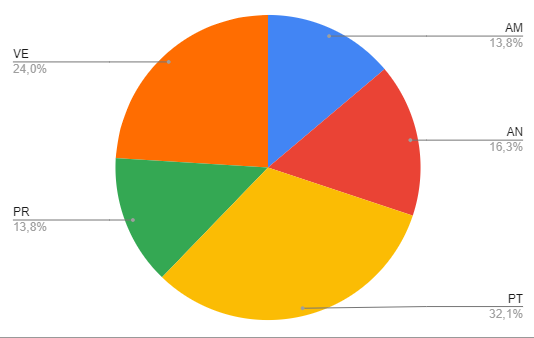
\includegraphics[width=0.8\linewidth]{../immagini/pdp/torta_suddvisione_lavoro_rendicontate_consuntivo.png}
		\caption{Grafico a torta della ripartizione dei costi per ruolo totali
			rendicontate}
	\end{center}
\end{figure}

\subsection{Prospetto suddivisione lavoro}\label{ConsuntivoOreRendicontateProspettoSuddivisioneLavoro}

Nella seguente tabella sono riportate le ore di impegno individuale rendicontate:
\quad
\def\tabularxcolumn#1{m{#1}}
{\rowcolors{2}{RawSienna!90!RawSienna!20}{RawSienna!70!RawSienna!40}
	
	\begin{center}
		\renewcommand{\arraystretch}{1.4}
		\begin{tabularx}{\textwidth}{|X|c|c|c|c|c|c|c|}
			\hline
			\rowcolor{airforceblue}
			\textbf{Nominativo} & \textbf{Re} & \textbf{Am} & \textbf{An} & \textbf{Pt} & \textbf{Pr} & \textbf{Ve} & \textbf{Totale ore}\\
			\hline
			\textit{Andrea Dorigo} & 21(-2) & 8 & 8(+3) & 22(-1) & 21 & 25 & 105\\
			\hline
			\textit{Margherita Mitillo} & 9 & 19 & 4(-5) & 23(+3) & 21(+2) & 29 & 105\\
			\hline
			\textit{Igli Mezini} & 19 & 10 & 14 & 22 & 10 & 30 & 105\\
			\hline
			\textit{Andrea Cecchin} & 7 & 11(-11) & 15(+11) & 28(+9) & 21(-9) & 23 & 105\\
			\hline
			\textit{Emma Roveroni} & 6 & 15 & 6 & 33(+9) & 18(-9) & 27 & 105\\
			\hline
			\textit{Alfredo Graziano} & 16 & 10 & 16(+1) & 22(-4) & 10 & 31(+3) & 105\\
			\hline
			\textit{Mattia Cocco} & 6 & 10 & 15(+7) & 25(+4) & 21(-11) & 28 & 105\\
			\hline
		\end{tabularx}
		\captionof{table}{\textbf{Consuntivo delle ore rendicontate}}
	\end{center}

	Come si può notare, la distribuzione oraria totale risulta uniforme tra tutti i componenti del gruppo.
	Le oscillazioni a consuntivo rispetto a quelle preventivate in alcuni casi sono state più significative, come nei ruoli di \textit{Analista}, \textit{Progettista} e \textit{Programmatore}, questo si è verificato perché durante lo svolgimento del progetto sono sorte delle situazioni che ci hanno portato a dover svolgere più alcuni ruoli rispetto ad altri.


	Il seguente istogramma riassume i dati ottenuti:
	\begin{figure}[!ht]
		\begin{center}
			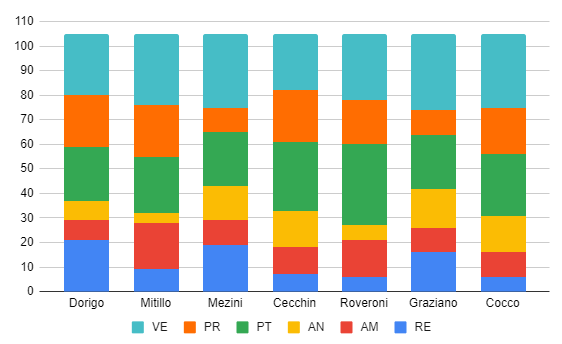
\includegraphics[width=0.8\linewidth]{../immagini/pdp/istogramma_rendicontate_consuntivo.png}
			\caption{Istogramma della ripartizione oraria rendicontate ottenute}
		\end{center}
	\end{figure}

% \def\tabularxcolumn#1{m{#1}}
% {\rowcolors{2}{RawSienna!90!RawSienna)!20}{RawSienna!70!RawSienna!40}
%
% 	\begin{center}
% 		\renewcommand{\arraystretch}{1.4}
% 		\begin{tabularx}{\textwidth}{|X|c|c|c|c|c|c|c|}
% 			\hline
% 			\rowcolor{airforceblue}
% 			\textbf{Incremento} & \textbf{Re} & \textbf{Am} & \textbf{An} & \textbf{Pt} & \textbf{Pr} & \textbf{Ve} & \textbf{Totale ore}\\
% 			\hline
% 			\textit{Incremento 3} & 2(+0) & 3(+0) & 0(+0) & 7(+0) & 16(+3) & 0(+0) & 28(+3)\\
% 			\hline
% 			\textit{Incremento 4} & 8(+3) & 6(+0) & 14(+7) & 0(+0) & 0(+0) & 20(+4) & 48(+14) \\
% 			\hline
% 			\textit{Incremento 5} & 2(+0) & 4(+0) & 0(+0) & 11(+0) & 21(+3) & 0(+0) & 38(+3)\\
% 			\hline
% 			\textit{Incremento 6} & 1(+0) & 2(+0) & 0(+0) & 2(+0) & 4(+0) & 0(+0) & 9(+0)\\
% 			\hline
% 			\textit{Incremento 7} & 1(+0) & 2(+0) & 0(+0) & 1(+0) & 3(+0) & 0(+0) & 7(+0)\\
% 			\hline
% 			\textit{Incremento 8} & 5(+0) & 6(+0) & 0(+0) & 5(+0) & 13(+0) & 0(+0) & 29(+0)\\
% 			\hline
% 			\textit{Incremento 9} & 8(+2) & 7(+0) & 0(+0) & 13(+0) & 0(+0) & 16(+0) & 44(+2)\\
% 			\hline
% 			Totale ore ruolo & 27(+5) & 30(+0) & 14(+7) & 39(+0) & 57(+6) & 36(+4) & 203(+22)\\
% 			\hline
% 		\end{tabularx}
% 		\captionof{table}{\textbf{Ore risultanti degli incrementi del secondo periodo della fase di Progettazione di dettaglio e codifica}}
% 	\end{center}
% 		\end{tabularx}
% 		\captionof{table}{\textbf{Ore risultanti degli incrementi del primo periodo della fase di Progettazione di dettaglio e codifica}}
% 	\end{center}
% %
% \subsubsection{Consuntivo}\label{ConsuntivoPrimoPeriodoDiProgettazioneDiDettaglioCodificaIncrementiCosto}
%
% \quad
% \def\tabularxcolumn#1{m{#1}}
% {\rowcolors{2}{RawSienna!90!RawSienna!20}{RawSienna!70!RawSienna!40}
% 	\begin{center}
% 		\renewcommand{\arraystretch}{1.4}
% 		\begin{tabularx}{10cm}{|X|c|c|}
% 			\hline
% 			\rowcolor{airforceblue}
% 			\textbf{Ruolo} & \textbf{Ore} & \textbf{Costo}\\
% 			\hline
% 			Responsabile & 8(+0) & 240\euro(+0\euro)\\
% 			\hline
% 			Amministratore & 11(+8) & 220\euro(+160\euro)\\
% 			\hline
% 			Analista & 0(-19) & 0\euro(-475\euro)\\
% 			\hline
% 			Progettista & 20(+0) & 440\euro(+0\euro)\\
% 			\hline
% 			Programmatore & 25(+5) & 375\euro(+75\euro)\\
% 			\hline
% 			Verificatore & 14(+0) & 210\euro(+0\euro)\\
% 			\hline
% 			\textbf{Totale Preventivo} & \textbf{84} & \textbf{1725\euro}\\
% 			\hline
% 			\textbf{Totale Consuntivo} & \textbf{78} & \textbf{1485\euro}\\
% 			\hline
% 			\textbf{Differenza} & \textbf{-6} & \textbf{-240\euro}
% 		\end{tabularx}
% 		\captionof{table}{\textbf{Consuntivo del primo periodo}}
% 	\end{center}
%
% \subsubsection{Conclusioni}\label{ConsuntivoPrimoPeriodoDiProgettazioneDiDettaglioCodificaConclusioni}
% 	Come emerso dalla tabella precedente, il bilancio per questo periodo risulta positivo in quanto è stato impiegato meno tempo del previsto per il ruolo di \textit{Analista}, erroneamente preventivato nell' incremento 1 dato che per le modifiche all'\textit{Analisi dei Requisiti} si è deciso di aspettare la valutazione e le indicazioni del committente$_G$.
% 	Invece nel ruolo di \textit{Amministratore} sono state impiegate più ore perché c'è stato molto lavoro per ristrutturare il codice prodotto per il Proof of Concecpt$_G$ e questa figura è indispensabile per l'efficienza e l'operatività dell'ambiente di sviluppo.
%
% \subsubsection{Ragionamento sugli scostamenti}\label{ConsuntivoPrimoPeriodoDiProgettazioneDiDettaglioCodificaRagionamentoScostamenti}
% 	Quello che emerge dagli scostamenti tra le ore preventivate e quelle in consuntivo fa notare subito che le ore preventivate in più nel ruolo di \textit{Analista} potevano essere evitate con uno studio più approfondito in fase di pianificazione.
% 	Per quanto riguarda il ruolo di \textit{Amministratore} invece risultano più ore in quanto si è deciso di andare il più avanti possibile con la codifica, sperando di poterle recuperare nei periodi successivi.
%
%
% \subsubsection{Preventivo a finire}\label{ConsuntivoPrimoPeriodoDiProgettazioneDiDettaglioCodificaPreventivoFinire}
% 	Il preventivo a finire di questo primo periodo presenta una diminuzione di 240\euro, il che è un dato positivo se preso singolarmente ma, nel nostro caso, le ore mancanti potrebbero aggiungersi al periodo successivo. Terremo monitorato il lavoro per riuscire a mantenere il risparmio maturato in questo periodo per tutta la fase di Progettazione di dettaglio e codifica.
%
% \subsection{Secondo periodo - dal 2021-03-23 al 2021-04-06 }\label{ConsuntivoSecondoPeriodoDiProgettazioneDiDettaglioCodifica}
%
% \subsubsection{Bilancio degli incrementi}\label{ConsuntivoSecondoPeriodoDiProgettazioneDiDettaglioCodificaIncrementi}
%
% 	La seguente tabella indica le ore effettivamente investite in ogni ruolo per il completamento di ciascun incremento di questo periodo e la differenza con quelle preventivate.
%
% \quad
% \def\tabularxcolumn#1{m{#1}}
% {\rowcolors{2}{RawSienna!90!RawSienna!20}{RawSienna!70!RawSienna!40}
%
% 	\begin{center}
% 		\renewcommand{\arraystretch}{1.4}
% 		\begin{tabularx}{\textwidth}{|X|c|c|c|c|c|c|c|}
% 			\hline
% 			\rowcolor{airforceblue}
% 			\textbf{Incremento} & \textbf{Re} & \textbf{Am} & \textbf{An} & \textbf{Pt} & \textbf{Pr} & \textbf{Ve} & \textbf{Totale ore}\\
% 			\hline
% 			\textit{Incremento 3} & 2(+0) & 3(+0) & 0(+0) & 7(+0) & 16(+3) & 0(+0) & 28(+3)\\
% 			\hline
% 			\textit{Incremento 4} & 8(+3) & 6(+0) & 14(+7) & 0(+0) & 0(+0) & 20(+4) & 48(+14) \\
% 			\hline
% 			\textit{Incremento 5} & 2(+0) & 4(+0) & 0(+0) & 11(+0) & 21(+3) & 0(+0) & 38(+3)\\
% 			\hline
% 			\textit{Incremento 6} & 1(+0) & 2(+0) & 0(+0) & 2(+0) & 4(+0) & 0(+0) & 9(+0)\\
% 			\hline
% 			\textit{Incremento 7} & 1(+0) & 2(+0) & 0(+0) & 1(+0) & 3(+0) & 0(+0) & 7(+0)\\
% 			\hline
% 			\textit{Incremento 8} & 5(+0) & 6(+0) & 0(+0) & 5(+0) & 13(+0) & 0(+0) & 29(+0)\\
% 			\hline
% 			\textit{Incremento 9} & 8(+2) & 7(+0) & 0(+0) & 13(+0) & 0(+0) & 16(+0) & 44(+2)\\
% 			\hline
% 			Totale ore ruolo & 27(+5) & 30(+0) & 14(+7) & 39(+0) & 57(+6) & 36(+4) & 203(+22)\\
% 			\hline
% 		\end{tabularx}
% 		\captionof{table}{\textbf{Ore risultanti degli incrementi del secondo periodo della fase di Progettazione di dettaglio e codifica}}
% 	\end{center}
%
% \subsubsection{Consuntivo}\label{ConsuntivoSecondoPeriodoDiProgettazioneDiDettaglioCodificaIncrementiCosto}
%
% 	\quad
% 	\def\tabularxcolumn#1{m{#1}}
% 	{\rowcolors{2}{RawSienna!90!RawSienna!20}{RawSienna!70!RawSienna!40}
% 		\begin{center}
% 			\renewcommand{\arraystretch}{1.4}
% 			\begin{tabularx}{10cm}{|X|c|c|}
% 				\hline
% 				\rowcolor{airforceblue}
% 				\textbf{Ruolo} & \textbf{Ore} & \textbf{Costo}\\
% 				\hline
% 				Responsabile & 27(+5) & 810\euro(+150\euro)\\
% 				\hline
% 				Amministratore & 30(+0) & 600\euro(+0\euro)\\
% 				\hline
% 				Analista & 14(+7) & 350\euro(+175\euro)\\
% 				\hline
% 				Progettista & 39(+0) & 858\euro(+0\euro)\\
% 				\hline
% 				Programmatore & 57(+6) & 855\euro(+90\euro)\\
% 				\hline
% 				Verificatore & 36(+4) & 540\euro(+60\euro)\\
% 				\hline
% 				\textbf{Totale Preventivo} & \textbf{181} & \textbf{3538\euro}\\
% 				\hline
% 				\textbf{Totale Consuntivo} & \textbf{203} & \textbf{4013\euro}\\
% 				\hline
% 				\textbf{Differenza} & \textbf{+22} & \textbf{475\euro}
% 			\end{tabularx}
% 			\captionof{table}{\textbf{Consuntivo del secondo periodo}}
% 		\end{center}
%
% 	\subsubsection{Conclusioni}\label{ConsuntivoSecondoPeriodoDiProgettazioneDiDettaglioCodificaConclusioni}
% 		In questo periodo, come emerge dalla tabella, il bilancio risulta negativo e questo è dovuto alle ore di differenza impiegate dalle seguenti figure:
% 		\begin{itemize}
% 			\item \textit{Responsabile}: in quanto sono state necessarie più ore per correggere ed ampliare il \textit{Piano di Progetto};
% 			\item \textit{Analista}: come intuito nel consuntivo del periodo precedente sono state necessarie più ore in questo ruolo in quanto la correzione dell'\textit{Analisi dei Requisiti} è stata effettuata in questo periodo;
% 			\item \textit{Programmatore}: in quanto sono state necessarie più ore nello sviluppo del front-end$_{\scaleto{G}{3pt}}$ e nell'elaborazione del modello di machine learning$_{\scaleto{G}{3pt}}$ come si vede dalla tabella degli incrementi;
% 			\item \textit{Verificatore}: in quanto la verifica dell'\textit{Analisi dei Requisiti} non era prevista in questo periodo.
% 		\end{itemize}
%
% 		\subsubsection{Ragionamento sugli scostamenti}\label{ConsuntivoSecondoPeriodoDiProgettazioneDiDettaglioCodificaRagionamentoScostamenti}
% 		Lo scostamento nel ruolo di \textit{Analista} riflette il ragionamento già fatto nel consuntivo del periodo precedente.
% 		Invece, il surplus di ore nel ruolo di \textit{Responsabile} ha fatto emergere una poca attenzione iniziale nella stesura del \textit{Piano di Progetto} che si è cercato di colmare in questa fase.
%
% 		\subsubsection{Preventivo a finire}\label{ConsuntivoSecondoPeriodoDiProgettazioneDiDettaglioCodificaPreventivoFinire}
% 		Il preventivo a finire presenta un surplus di 475\euro.
% 		Purtroppo non siamo riusciti a mantenere il risparmio ottenuto nel periodo precedente in quanto il surplus di ore consuntivate nei ruoli riportati sopra è maggiore delle ore risparmiate nel ruolo di \textit{Analista} nel periodo precedente.
%
% \subsection{Terzo periodo - dal 2021-04-07 al 2021-04-29} }\label{ConsuntivoTerzoPeriodoDiProgettazioneDiDettaglioCodifica}
%
% \subsubsection{Bilancio degli incrementi}\label{ConsuntivoTerzoPeriodoDiProgettazioneDiDettaglioCodificaIncrementi}
%
% La seguente tabella indica le ore effettivamente investite in ogni ruolo per il completamento di ciascun incremento di questo periodo e la differenza con quelle preventivate.
%
% \quad
% \def\tabularxcolumn#1{m{#1}}
% {\rowcolors{2}{RawSienna!90!RawSienna!20}{RawSienna!70!RawSienna!40}
%
% 	\begin{center}
% 		\renewcommand{\arraystretch}{1.4}
% 		\begin{tabularx}{\textwidth}{|X|c|c|c|c|c|c|c|}
% 			\hline
% 			\rowcolor{airforceblue}
% 			\textbf{Incremento} & \textbf{Re} & \textbf{Am} & \textbf{An} & \textbf{Pt} & \textbf{Pr} & \textbf{Ve} & \textbf{Totale ore}\\
% 			\hline
% 			\textit{Incremento 10} & 3(+0) & 3(+0) & 16(+16) & 8(+0) & 0(+0) & 30(+0) & 60(+16)\\
% 			\hline
% 			\textit{Incremento 11} & 2(+0) & 2(+0) & 0(+0) & 2(+0) & 0(+0) & 0(+0) & 6(+0)\\
% 			\hline
% 			Totale ore ruolo & 5(+0) & 5(+0) & 0(+16) & 10(+0) & 0(+0) & 30(+0) & 66(+16)\\
% 			\hline
% 		\end{tabularx}
% 		\captionof{table}{\textbf{Ore risultanti degli incrementi del terzo periodo della fase di Progettazione di dettaglio e codifica}}
% 	\end{center}
%
%
% 	\subsubsection{Consuntivo}\label{ConsuntivoTerzoPeriodoDiProgettazioneDiDettaglioCodificaIncrementiCosto}
%
% 	\quad
% 	\def\tabularxcolumn#1{m{#1}}
% 	{\rowcolors{2}{RawSienna!90!RawSienna!20}{RawSienna!70!RawSienna!40}
% 		\begin{center}
% 			\renewcommand{\arraystretch}{1.4}
% 			\begin{tabularx}{10cm}{|X|c|c|}
% 				\hline
% 				\rowcolor{airforceblue}
% 				\textbf{Ruolo} & \textbf{Ore} & \textbf{Costo}\\
% 				\hline
% 				Responsabile & 5(+0) & 150\euro(+0\euro)\\
% 				\hline
% 				Amministratore & 5(+0) & 100\euro(+0\euro)\\
% 				\hline
% 				Analista & 16(+16) & 400\euro(+400\euro)\\
% 				\hline
% 				Progettista & 10(+0) & 220\euro(+0\euro)\\
% 				\hline
% 				Programmatore & 0(+0) & 0\euro(+0\euro)\\
% 				\hline
% 				Verificatore & 30(+0) & 450\euro(+0\euro)\\
% 				\hline
% 				\textbf{Totale Preventivo} & \textbf{50} & \textbf{920\euro}\\
% 				\hline
% 				\textbf{Totale Consuntivo} & \textbf{66} & \textbf{1320\euro}\\
% 				\hline
% 				\textbf{Differenza} & \textbf{+16} & \textbf{+400\euro}
% 			\end{tabularx}
% 			\captionof{table}{\textbf{Consuntivo del terzo periodo}}
% 		\end{center}
%
% \subsubsection{Conclusioni}\label{ConsuntivoTerzoPeriodoDiProgettazioneDiDettaglioCodificaConclusioni}
% Come emerso dalla tabella precedente, il bilancio risulta negativo in quanto abbiamo dovuto impiegare più ore nel ruolo di \textit{Analista} rispetto alle ore preventivate. Sono stati riscontrati vari errori da parte del committente$_{\scaleto{G}{3pt}}$ nel documento legato all'\textit{Analisi dei Requisiti} che ha portato ad una rivisitazione profonda di quest'ultimo.
%
%
% \subsubsection{Ragionamento sugli scostamenti}\label{ConsuntivoTerzoPeriodoDiProgettazioneDiDettaglioCodificaRagionamentoScostamenti}
% Purtroppo anche in questo periodo il ruolo di \textit{Analista} ha subito una maggiorazione per i motivi riportati sopra.
%
% \subsubsection{Preventivo a finire}\label{ConsuntivoTerzoPeriodoDiProgettazioneDiDettaglioCodificaPreventivoFinire}
% Il preventivo a finire di questo periodo presenta quindi un surplus di 400\euro.
%
% \subsection{Consuntivo complessivo delle fasi}\label{ConsuntivoPeriodoDiProgettazioneDettaglioCodificaComplessivoDelleFasi}
%
% 			Nella tabella successiva viene descritto il calcolo delle ore totali di tutte le parti precedentemente descritte.
%
% 			\quad
% 			\def\tabularxcolumn#1{m{#1}}
% 			{\rowcolors{2}{RawSienna!90!RawSienna!20}{RawSienna!70!RawSienna!40}
% 				\begin{center}
% 					\renewcommand{\arraystretch}{1.4}
% 					\begin{tabularx}{10cm}{|X|c|c|}
% 						\hline
% 						\rowcolor{airforceblue}
% 						\textbf{Ruolo} & \textbf{Ore} & \textbf{Costo}\\
% 						\hline
% 						Responsabile & 40(+5) & 1200\euro(+150\euro)\\
% 						\hline
% 						Amministratore & 46(+8) & 920\euro(+160\euro)\\
% 						\hline
% 						Analista & 33(+4) & 825\euro(+100\euro)\\
% 						\hline
% 						Progettista & 64(+0) & 1518\euro(+0\euro)\\
% 						\hline
% 						Programmatore & 82(+11) & 1230\euro(+165\euro)\\
% 						\hline
% 						Verificatore & 74(+4) & 1200\euro(+60\euro)\\
% 						\hline
% 						\textbf{Totale Preventivo} & \textbf{315} & \textbf{6183\euro}\\
% 						\hline
% 						\textbf{Totale Consuntivo} & \textbf{346} & \textbf{6818\euro}\\
% 						\hline
% 						\textbf{Differenza} & \textbf{31} & \textbf{635\euro}
% 					\end{tabularx}
% 					\captionof{table}{\textbf{Consuntivo complessivo delle fasi}}
% 				\end{center}

% \subsection{Conclusioni}\label{ConsuntivoPeriodoDiProgettazioneDettaglioCodificaConclusioni}
% Come emerge dalla tabella, il bilancio dell'intera fase risulta negativo e questo è dovuto alle ore di differenza impiegate dalle seguenti figure:
% \begin{itemize}
% 	\item \textit{Responsabile}: in quanto sono state necessarie più ore per correggere ed ampliare il \textit{Piano di Progetto} oltre alle ore impiegate a svolgere gli altri compiti di sua competenza;
% 	\item \textit{Analista}: le ore preventivare per questo ruolo in questa fase si sono rivelate tutte necessarie in quanto il documento \textit{Analisi dei Requisiti} ha subito più di una correzione;
% 	\item \textit{Programmatore}: i motivi principali sono stati il completamento del modello di machine learning$_{\scaleto{G}{3pt}}$ e il collegamento della web-app al backend$_{\scaleto{G}{3pt}}$;
% 	\item \textit{Amministratore}: in quanto la ristrutturazione del codice prodotto per il Proof of Concept$_{\scaleto{G}{3pt}}$ ha richiesto qualche ora in più.
% \end{itemize}
%
% \subsection{Preventivo a finire}\label{ConsuntivoPeriodoDiProgettazioneDettaglioCodificaPreventivoAFinire}
% Il preventivo a finire di questa intera fase risulta quindi con un surplus di 635\euro, portando il totale a  15955\euro, nonostante questo importo sia maggiore di quanto preventivato il gruppo ha concluso tutti gli incrementi previsti per questa fase e ha soddisfatto tutti i requisiti obbligatori individuati nell'\textit{Analisi dei Requisiti v4.0.0}. Crediamo che nella prossima fase rinunceremo ad implementare alcuni dei requisiti desiderabili ed opzionali per non aggravare ulteriormente il preventivo a finire.
